\documentclass[10pt,a4paper]{article}

% =========================================================
% PACKAGES
% =========================================================

\usepackage[margin=0.75in]{geometry}
\usepackage{graphicx}
\usepackage{booktabs}
\usepackage{amsmath,amssymb}
\usepackage{xcolor}
\usepackage{microtype}
\usepackage{hyperref}
\usepackage{titlesec}
\usepackage{fancyhdr}
\usepackage{fontawesome5}
\usepackage{caption}

\usepackage{soul}

% =========================================================
% COLORS
% =========================================================

\definecolor{accent}{HTML}{5A4FCF}
\definecolor{textgray}{HTML}{444444}

% =========================================================
% LINKS
% =========================================================

\hypersetup{
    colorlinks=true,
    linkcolor=accent,
    citecolor=accent,
    urlcolor=accent
}

% =========================================================
% SECTION STYLE
% =========================================================

\titleformat{\section}
    {\large\bfseries\color{accent}}
    {\thesection.}
    {0.5em}
    {}

\titleformat{\subsection}
    {\normalsize\bfseries\color{textgray}}
    {\thesubsection}
    {0.5em}
    {}

\titlespacing*{\section}{0pt}{10pt}{4pt}
\titlespacing*{\subsection}{0pt}{7pt}{3pt}

% =========================================================
% GENERAL FORMATTING
% =========================================================

\setlength{\parindent}{0pt}
\setlength{\parskip}{4pt}

\captionsetup{
    font=small,
    labelfont=bf
}

% =========================================================
% HEADER / FOOTER
% =========================================================

\pagestyle{fancy}
\fancyhf{}

\lhead{\small Modern Computer Vision}
\rhead{\small Final Project}
\cfoot{\small \thepage}

\renewcommand{\headrulewidth}{0.3pt}

% =========================================================
% DOCUMENT
% =========================================================

\begin{document}

\begin{center}

    {\LARGE\bfseries
    Does Spatial Credit Survive the Reward Model?\\
    Auditing Region-Level Feedback in Instruction-Based Image Editing}

    \vspace{4pt}

    {\large\color{accent}
    Modern Computer Vision -- Final Project}

    \vspace{3pt}

    Noam Akkerman \quad $\cdot$ \quad
    Nadav Anolik \quad $\cdot$ \quad
    Anis Barhoum \quad $\cdot$ \quad
    Anna Kravets \quad $\cdot$ \quad
    Liad Livneh

    \vspace{7pt}

    {\small
    Faculty of Data and Decision Sciences\\
    Technion -- Israel Institute of Technology
    }
    \vspace{4pt}
    
    {\small
    \href{https://github.com/nadavanolik/mcv-spatial-audit}
    {\faGithub\ \texttt{GitHub Repo}}
    }

    

\end{center}

\vspace{4pt}
\hrule
\vspace{8pt}

% =========================================================
% ABSTRACT
% =========================================================

\begin{abstract}

Reinforcement-learning based methods for image editing increasingly reward each region of an edit separately, with scores from a vision-language model (VLM) judge, assuming that the score of a region reflects that region. We test this assumption with a controlled audit: we corrupt exactly one region of an edited image and ask the judge to score every region again. Applying the region-level prompt of SpatialFlow-GRPO to Qwen3-VL-8B and InternVL3-8B on 150 COCO photographs (5,236 variants), we find that while both judges perceive the damage, neither attributes it to the damaged region: the AUROC for singling it out is 0.52--0.54. The scores also depend more on the prompt than on the pixels. The judge receives the regions to score as a list, and showing it the same clean image with that list in a different order changes a region's score 1.6--1.8 times as much as corrupting that region does. These results bring us to believe that contrary to the RL methods' underlying assumption, per-region VLM rewards carry far less spatial information than their form implies.

\end{abstract}

% =========================================================
% INTRODUCTION
% =========================================================

\section{Introduction}

Recent reinforcement-learning methods for instruction-based image editing, all built on GRPO \cite{shao2024deepseekmath} or its flow-matching variant Flow-GRPO \cite{liu2025flowgrpo}, replace a single whole-image reward with region-level feedback from a VLM judge: SpatialFlow-GRPO \cite{yang2026spatialflow}, Edit-GRPO \cite{xu2026editgrpo}, Region-Constrained GRPO \cite{ouyang2026rcgrpo} and SpatialReward \cite{long2026spatialreward}. They assume that the score assigned to a region reflects that region. If it reflects the image as a whole instead, the reward gives misleading spatial credit while appearing localized. SpatialReward studies such failures through attention, we test them behaviourally.

We corrupt exactly one region of an edited image, leave the rest untouched, and ask the judge to score every region again. A spatially faithful judge lowers the corrupted region more than the others. Because we know where the damage is, the audit separates two abilities: detecting that the image degraded, and identifying where. Across two model families, we find the first without the second.

% =========================================================
% METHOD
% =========================================================

\section{Method}

\textbf{Benchmark.} We select COCO train2017 images \cite{lin2014coco} with 3--5 instances, each covering 2--25\% of the image, of distinct categories and with no other instance of those categories, so that an instruction such as ``make the car red'' is unambiguous: 150 photographs with 476 regions, each region being one object. Each region receives one templated instruction (a recolouring, a material or attribute change, or at most one removal per image); the instructions of an image are combined, and the image is edited once with FLUX.1-Kontext-dev \cite{bfl2025kontext} (28 steps, guidance 2.5, fixed seed). We then corrupt one region of the edit at a time, inside its COCO mask with a feathered edge ($\sigma=6$\,px), using five corruptions at a mild and a strong setting: blur ($\sigma=1.5$ / $7$\,px), Gaussian noise ($\sigma=6$ / $28$ grey levels), JPEG (quality 40 / 7), saturation ($\times1.4$ / $\times3$), and removal by inpainting \cite{telea2004inpainting} (radius 3 / 10\,px), reported as one condition because both settings delete the object. Each region yields ten corrupted variants plus the uncorrupted edit as its clean control, 5,236 images in total (Appendix~\ref{app:example}, Figure~\ref{fig:example}).

\textbf{Judges and scores.} We audit the region-level judging protocol of SpatialFlow-GRPO \cite{yang2026spatialflow}, i.e.\ its region-scoring prompt (its Appendix A.4.3) and reward formula. SpatialFlow-GRPO's own reward model is a fine-tuned Qwen3-VL-8B-Instruct. We apply it to the base Qwen3-VL-8B-Instruct \cite{bai2025qwen3vl} and to InternVL3-8B \cite{zhu2025internvl3}, a second family with its own vision encoder; we therefore audit the protocol, not the fine-tuned model. The judge is called twice per image. A \emph{consistency} call receives the source photograph, the edit, the instruction and the list of regions, each a label and a bounding box in the 0--1000 coordinates both models are trained on, and returns two scores per region on 0--25: \emph{success} (was the instruction carried out) and \emph{preserve} (was the rest of the region kept). A \emph{quality} call receives the edit alone and returns two image-level scores on 0--25: \emph{naturalness} (does it look natural) and \emph{artifacts} (25 = free of distortion, blur and similar defects). The consistency prompt is copied verbatim. The paper prints only the output of the quality call (its Appendix A.4.4), not its prompt, so we wrote one that asks for the same two scores; it also does not show how the regions are inserted into the prompt, so that formatting is ours. Outputs are constrained to a JSON schema and decoded greedily. Following the paper's Equation (3), the reward of region $r$ is
\[
\phi_r = \min(\mathrm{success}_r, \mathrm{preserve}_r), \qquad
\mathrm{AES} = \min(\mathrm{naturalness}, \mathrm{artifacts}), \qquad
R_r = \sqrt{\phi_r \cdot \mathrm{AES}}\,/\,25 .
\]
AES, the image-level quality score, is shared by every region of the image, so we use it to test whether the judge perceives the damage, and $\phi$, the only term that can tell regions apart, to test where it attributes it. For each region, $\Delta\phi = \phi^{\mathrm{corrupt}} - \phi^{\mathrm{clean}}$ against the clean control of the same image.

\textbf{Analyses.} \emph{Perception:} $\Delta$AES per corruption, divided by the judge's between-photograph SD of clean AES so that the two judges' scales are comparable. \emph{Localization:} the AUROC of $-\Delta\phi$ separating corrupted from untouched regions, i.e.\ the probability that a corrupted region drops more than an untouched one (0.5 = chance, ties count half). Since ties are common, we also report the share of regions whose $\phi$ did not move. Regions already at $\phi=0$ cannot drop and are excluded (\emph{floor-excluded}). \emph{Coupling:} when one region is damaged, do the untouched regions move together, as if driven by one verdict on the whole image? If the judge scores each region on its own, a corrupted variant should often change some regions and not others; if it scores the image as a whole, the regions change all together or not at all. We therefore count the variants in which only some regions change, and compare with the count expected if regions changed independently (a permutation test that keeps each region's own rate of change). We also measure how well the mean $\Delta\phi$ of the other untouched regions predicts an untouched region's $\Delta\phi$ ($R^2$, 0 if independent). \emph{Nuisance:} does the score move when only the request changes? On the 476 clean edits, we reorder the list of regions, drop one other region from it, or draw the boxes on both images as well as listing them, and divide the mean $|\Delta\phi|$ by that caused by damage to the corrupted region, averaged over all corruptions and both settings. A ratio above 1 means the change moves the score more than damage does, below 1 less. \emph{Exploitability:} can the reward rise without a better edit? We judge the clean edits with no images, or after sharpening the whole edit or only one region's box, and measure the gain on edits the judge called failed (success $<20$), where there is room to gain. Edits picked for a low score tend to score higher when re-judged, so we also pick them with the \emph{other} judge. \emph{Noise floor:} how much does the score move when nothing changes? A photograph's clean controls are identical requests, yet greedy decoding in vLLM \cite{kwon2023vllm} is not bit-reproducible, so the differences between their answers set the level any real effect must exceed. All 95\% intervals resample the 150 photographs (1,000 bootstrap draws \cite{efron1993bootstrap}) and are not corrected for multiple comparisons.

% =========================================================
% RESULTS
% =========================================================

\section{Results}

Both judges return a valid answer for every request. Identical requests leave $\phi$ unchanged 97\% (Qwen) and 91\% (InternVL) of the time, and damage moves the corrupted region's $\phi$ 4--6 times as much as this floor.

\begin{figure}[t]
\centering
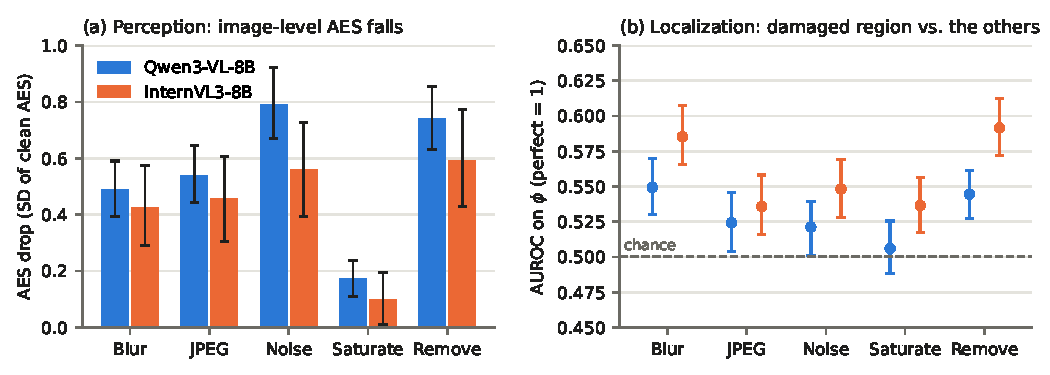
\includegraphics[width=\linewidth]{figures/fig_perception_localization.pdf}
\caption{Perception against localization at the strong setting of each corruption (removal is a single condition). (a) Drop in image-level AES after corrupting one region, in between-photo SDs of clean AES. (b) Floor-excluded AUROC on $\phi$ (0.5 = chance, 1 = perfect). Error bars: 95\% bootstrap over photographs.}
\label{fig:perloc}
\end{figure}

\textbf{Both judges perceive the damage.} Every strong corruption lowers AES with an interval below zero (Figure~\ref{fig:perloc}a; both settings in Appendix~\ref{app:tables}). Strong noise and removal have the largest effect, and the mild settings are barely noticed. Qwen reacts more: strong noise moves its AES by 0.79 between-photo SDs, against 0.56 for InternVL.

\begin{table}[t]
\centering
\small
\begin{tabular}{llccccc}
\toprule
 & & & \multicolumn{2}{c}{unchanged} & \multicolumn{2}{c}{mean $\Delta\phi$} \\
\cmidrule(lr){4-5}\cmidrule(lr){6-7}
Judge & Damage & AUROC & corrupted & untouched & corrupted & untouched \\
\midrule
Qwen3-VL-8B  & Mild    & 0.511 & 82\% & 83\% & $-0.60$ & $-0.45$ \\
             & Strong  & 0.525 & 75\% & 78\% & $-1.26$ & $-0.69$ \\
             & Removal & 0.545 & 63\% & 71\% & $-3.00$ & $-1.67$ \\
             & All     & 0.523 & 75\% & 79\% & $-1.34$ & $-0.79$ \\
\midrule
InternVL3-8B & Mild    & 0.506 & 79\% & 78\% & $-0.39$ & $-0.21$ \\
             & Strong  & 0.550 & 67\% & 71\% & $-1.77$ & $-0.85$ \\
             & Removal & 0.592 & 55\% & 65\% & $-3.79$ & $-1.54$ \\
             & All     & 0.541 & 69\% & 73\% & $-1.62$ & $-0.73$ \\
\bottomrule
\end{tabular}
\caption{Localization on $\phi$, floor-excluded. Mild and Strong pool blur, JPEG, noise and saturation. AUROC: the probability that a randomly chosen corrupted region's $\phi$ drops more than a randomly chosen untouched region's (0.5 = chance, 1 = perfect). Unchanged: share of regions whose $\phi$ did not move. A judge that localizes damage gives AUROC near 1, rarely leaves the corrupted region unchanged, and leaves untouched regions at $\Delta\phi \approx 0$. Qwen: 131 photographs, 11,880 region scores; InternVL: 136, 11,010.}
\label{tab:localization}
\end{table}

\textbf{Neither judge localizes it.} Overall AUROC is 0.523 for Qwen and 0.541 for InternVL, and the corrupted region keeps exactly the same $\phi$ nearly as often as the untouched regions do (Table~\ref{tab:localization}). Localization does not follow perception (Figure~\ref{fig:perloc}b): strong noise is what Qwen perceives most, yet one of the corruptions it localizes least (0.521), and InternVL localizes every corruption slightly better than Qwen while perceiving each one less. No corruption reaches 0.6. The result holds when we drop untouched regions whose box the corrupted pixels reach (0.521 and 0.539), on photographs whose edit did not move objects away from the source masks (0.525 and 0.544), and, for Qwen, with box coordinates in pixels instead of 0--1000 (AUROC 0.519 vs.\ 0.523, difference within $[-0.009, +0.018]$). Appendix~\ref{app:example} shows the failure on one photograph.

\textbf{Regions move together.} The share of variants in which only some regions change is 4.5 percentage points below what independent regions would give for Qwen $[-5.8, -3.2]$, and 6.5 below for InternVL $[-8.6, -4.7]$. An untouched region's $\Delta\phi$ is partly predicted by the other untouched regions' ($R^2 = 0.14$ $[0.07, 0.23]$ and $0.19$ $[0.10, 0.31]$). The coupling is modest but nonzero, and since $\phi$ excludes AES, it is not an artifact of the reward formula.

\textbf{The order of the region list moves the score more than damage.} Reordering the list moves $\phi$ 1.60 $[1.23, 2.09]$ (Qwen) and 1.80 $[1.48, 2.22]$ (InternVL) times as much as corrupting the region, averaged over all corruptions and settings; dropping another region from the list, 1.68 and 1.47 times; drawing the boxes on the images, 0.95 and 1.89 times (Appendix~\ref{app:tables}). Random reorderings that happened to keep the original order send identical requests and move at the noise floor (mean $|\Delta\phi|$ 0.30 vs.\ 3.54 for reordered lists, Qwen), so the order itself is the cause.

\textbf{Without the images, failed edits score higher.} With no image, both judges fall back to a high, nearly constant default (mean reward 0.75 and 0.73 against 0.64 and 0.55 with the images; SD 0.09 and 0.13). Edits the judge had scored as failed therefore gain about $+0.45$, and the gain holds when the other judge selects them ($+0.27$ $[0.21, 0.33]$ and $+0.38$ $[0.33, 0.44]$). Cosmetic enhancement gives no gain, globally or inside the target box.

% =========================================================
% DISCUSSION
% =========================================================

\section{Discussion}

Both judges see the damage, but the per-region score does not follow where it is, in two model families of the same size. The score appears to track a verdict on the image as a whole, plus how the request is formatted. Regions move together on $\phi$, which excludes the shared image term; Qwen's $\phi$ is nearly binary (76\% of scores are exactly 0 or 25), so a local defect can surface as a jump on every region at once, with the judge inventing failures in undamaged regions (Appendix~\ref{app:example}); and the order of the list moves the score more than damage does. Each judge registers the damage well above its own noise floor, so the score is not arbitrary at the level of the image: what is missing is the assignment to a region. For training, such a reward delivers mostly image-level credit. A policy can be penalized in a region it handled correctly and receive no specific signal where it erred. Methods that rely on it could average over region orderings, and should run a check like ours, which needs no training and no labels, before trusting a judge with spatial credit.

\textbf{Limitations.} We audit the protocol with base models, not SpatialFlow-GRPO's fine-tuned reward model; fine-tuning on region-level labels may improve localization, and the same audit applies to it directly. The corruptions are synthetic rather than natural editing failures, regions cover 2--25\% of the image, decoding is greedy, and the 5,236 variants come from 150 photographs.

\bibliographystyle{plain}
\bibliography{references}


\clearpage
\appendix
\section{One photograph}
\label{app:example}

Figure~\ref{fig:heatmap} shows the failure on a single photograph. All three regions start at the maximum $\phi$ of 25. Strong noise on the person sends all three to 0. The same noise on the bench changes nothing, and on the potted plant it lowers only the person. The judge registers the damage, since AES drops by 5 points, but it does not place it. After the person is noised, its reasoning states that ``no moustache was added'' and that the potted plant ``remains fully visible in both images; it was not erased as instructed'', although both edits are untouched in that variant. A local corruption turns into a verdict that every edit failed. We picked this photograph as a clear case, not a typical one, from those where every region starts above $\phi=0$, AES dropped, and the untouched regions moved as much as the corrupted one. Table~\ref{tab:localization} gives the rates over the whole benchmark.

\begin{figure}[!h]
\centering
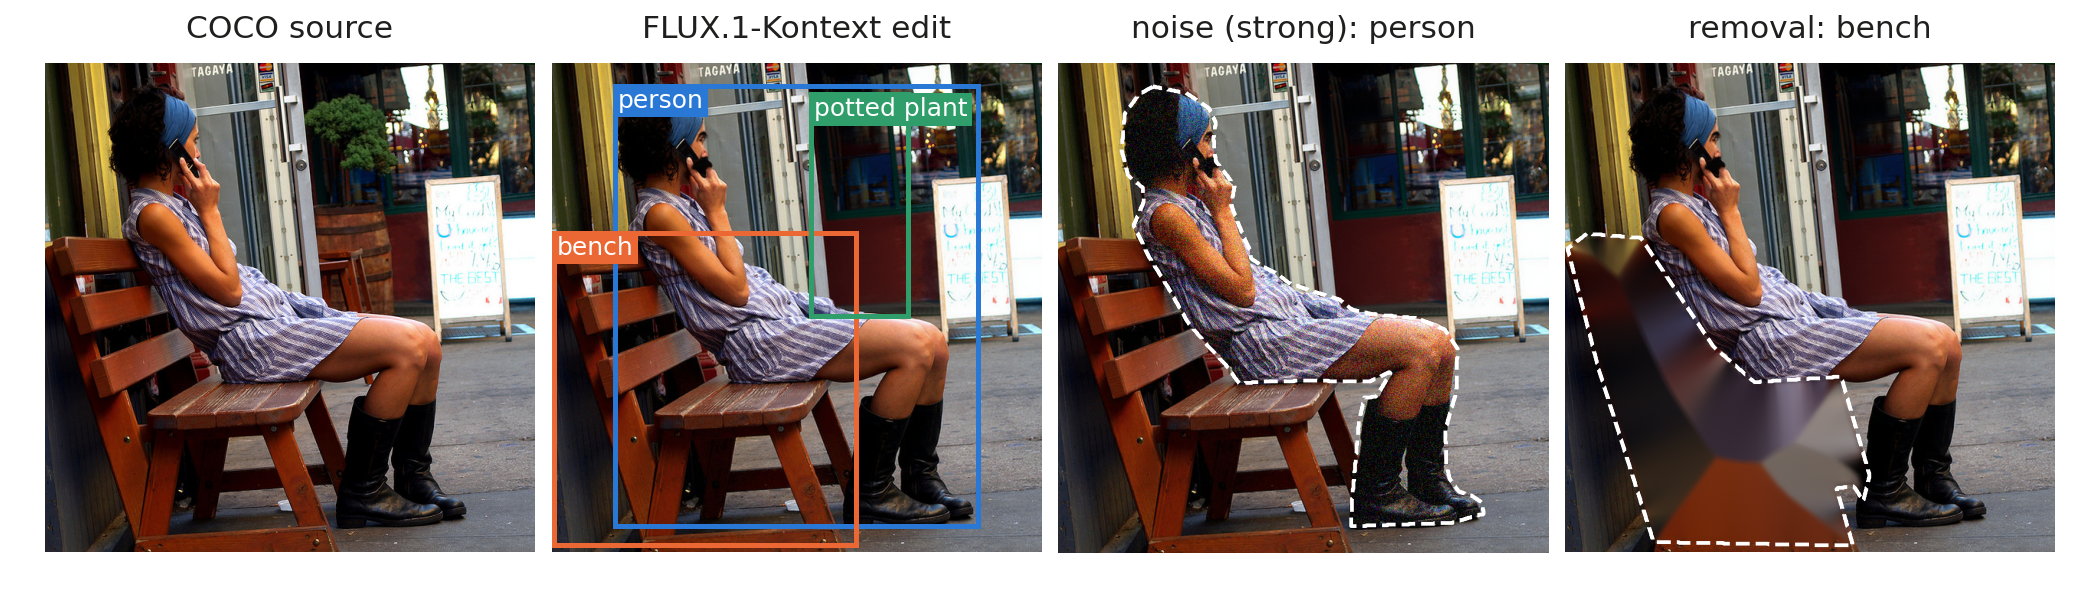
\includegraphics[width=\linewidth]{figures/fig_example_pipeline.png}
\caption{One benchmark photograph (COCO 381607). Instruction: ``add a moustache to the person, make the bench look like it is made of wood, erase the potted plant''. The boxes on the edit are the regions listed to the judge. Right: two of the photograph's 30 corrupted variants, strong noise on the person and removal of the bench; the dashed outline is the corrupted mask.}
\label{fig:example}
\end{figure}

\begin{figure}[!h]
\centering
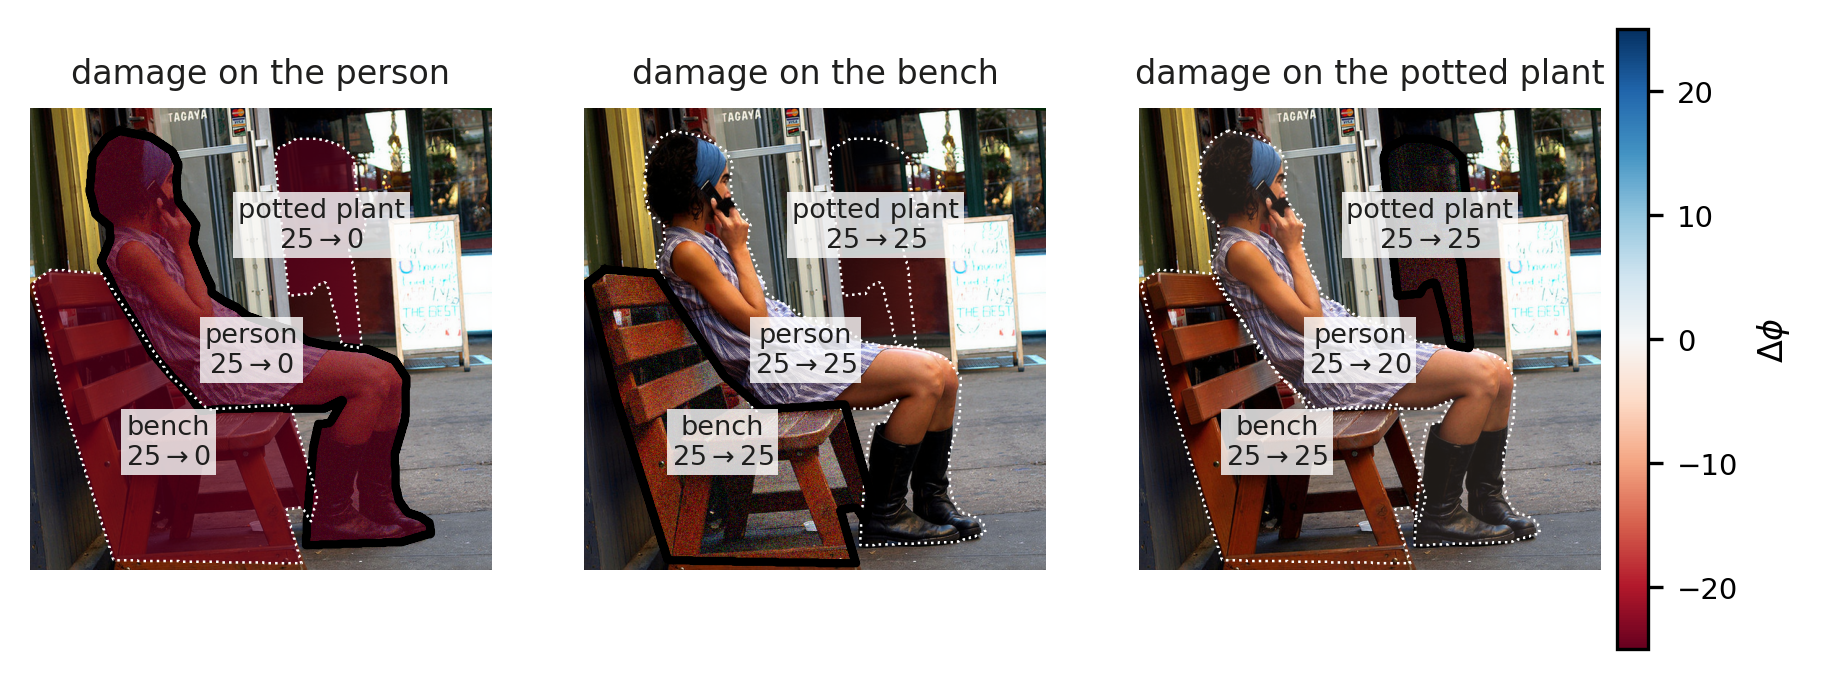
\includegraphics[width=\linewidth]{figures/fig_example_heatmap.png}
\caption{Qwen3-VL-8B's per-region score on the photograph of Figure~\ref{fig:example} under strong noise, one panel per corrupted region (black outline). Each region is tinted by its $\Delta\phi$ against the clean edit, and labelled with $\phi$ before $\to$ after. The potted plant was erased by the edit, so its mask marks where it stood.}
\label{fig:heatmap}
\end{figure}



\clearpage
\section{Perception and nuisance tables}
\label{app:tables}

Table~\ref{tab:perception} gives the image-level AES change at both settings of every corruption (Figure~\ref{fig:perloc}a shows the strong setting). Table~\ref{tab:nuisance} gives the nuisance ratios quoted in Section~3.

\begin{center}
\centering
\small
\begin{tabular}{lcccc}
\toprule
 & \multicolumn{2}{c}{Qwen3-VL-8B} & \multicolumn{2}{c}{InternVL3-8B} \\
\cmidrule(lr){2-3}\cmidrule(lr){4-5}
Corruption & mild & strong & mild & strong \\
\midrule
Blur       & $-0.51$ & $-1.62$ & $-0.16$ & $-0.68$ \\
JPEG       & $-0.09$ & $-1.79$ & $\phantom{-}0.00$ & $-0.73$ \\
Noise      & $\phantom{-}0.00$ & $-2.62$ & $-0.03$ & $-0.90$ \\
Saturation & $-0.19$ & $-0.57$ & $-0.04$ & $-0.16$ \\
Removal    & \multicolumn{2}{c}{$-2.45$} & \multicolumn{2}{c}{$-0.95$} \\
\midrule
Between-photo SD of clean AES & \multicolumn{2}{c}{3.31} & \multicolumn{2}{c}{1.60} \\
\bottomrule
\end{tabular}
\captionof{table}{Change in the image-level quality score AES (0--25) after corrupting one region, relative to the clean edit, at both settings. Strong noise: Qwen $-2.62$ $[-3.06, -2.22]$, InternVL $-0.90$ $[-1.16, -0.63]$.}
\label{tab:perception}
\end{center}

\begin{center}
\centering
\small
\begin{tabular}{lcc}
\toprule
Change to the request (the edit is clean) & Qwen3-VL-8B & InternVL3-8B \\
\midrule
Reorder the region list        & 1.60 $[1.23, 2.09]$ & 1.80 $[1.48, 2.22]$ \\
Drop one other region from the list & 1.68 $[1.25, 2.25]$ & 1.47 $[1.15, 1.86]$ \\
Draw the boxes on both images   & 0.95 $[0.64, 1.33]$ & 1.89 $[1.54, 2.30]$ \\
\bottomrule
\end{tabular}
\captionof{table}{Mean $|\Delta\phi|$ caused by each change on the clean edits, divided by the mean $|\Delta\phi|$ of the corrupted region under real damage, averaged over all five corruptions and both settings. Above 1: the change moves the score more than damage does; below 1: less. Floor-excluded, ratio of per-photograph means.}
\label{tab:nuisance}
\end{center}

\end{document}